% !TEX root = calculus.tex


\chapter{INTEGRAL}
\label{integral}

\athr We know already that the difference between the values of an antiderivative at two arbitrary points depends only on the choice of these points (and, evidently, on the type of the initial function $f (x))$. As these two points we choose points $a$ and $b$, that is, consider an increment of an antiderivative, $F (b) - F (a)$, This increment plays a very important role among the tools of calculus; it is called the \emph{integral}.
\begin{mytheo}{Definition}
The increment of an anti-derivative $F$ of a function $f$, i,e. $F(b)- F(a)$, is said to be the integral of $f$ from $a$ to $b$.
\end{mytheo}
The notation of the integral is:
\begin{equation*}%
\int_{a}^{b} f(x) \, dx
\end{equation*}
(it reads: ``integral of $f$ of $x$, $dx$, from $a$ to $b$''). The numbers $a$ and $b$ are the \emph{lower} and \emph{upper limits of integration}. The function $f$ is said to be \emph{integrand}, and $x$ the \emph{integration variable}.

Consequently, if $F$ is one of the antiderivatives of the function $f$, then the definition of an integral states that 
\begin{equation}%
\boxed{\int_{a}^{b} f(x) \, dx = F(b)- F(a)}
\label{newton-lebnitz-formula}
% eq 1 of 12
\end{equation}

Formula \eqref{newton-lebnitz-formula} is known in the literature on mathematics as the \emph{Newton-Leibnitz formula}. Remember that $F$ here is an arbitrary antiderivative of the function $f$.
\begin{figure}[!ht]%[13]{r}{0.5\textwidth}
\centering
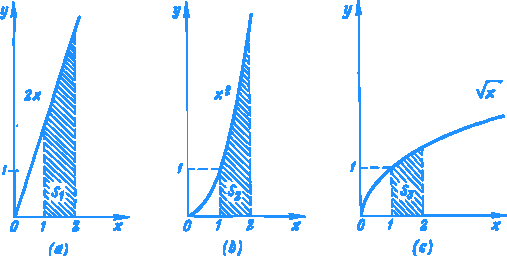
\includegraphics[width=.9\textwidth]{figures/fig-49.pdf}
\caption{Examining the geometrical interpretation of the integral as area.}
\label{fig-49}
\end{figure}

\rdr As far as I understand, the integral of the function $f$ from $a$ to $b$ is precisely the area of the curvilinear trapezoid bounded by the graph of the function $f (x)$ over the interval $[a, b]$. Is that right?

\athr Absolutely. The expression
\begin{equation*}%
\int_{a}^{b} f(x) \, dx
\end{equation*}
is nothing less than the area of this geometrical figure. \fig{fig-49} shows three cases plotting different integrands:
\begin{enumerate*}[label=(\alph*)]
\item $f(x) = 2x$, 
\item $f(x) = x^{2}$,
\item $f(x) = \sqrt{x}$. 
\end{enumerate*}

The limits of integration are chosen identical in all the three cases: $a = 1, \, b = 2$. The corresponding areas of the curvilinear trapezoids are shaded in the figure:
\begin{align*}%
S_{1} & = \int_{1}^{2} 2 x \, dx \\
S_{2} & = \int_{1}^{2} x^{2} \, dx \\
S_{3} & = \int_{1}^{2} \sqrt{x} \, dx
\end{align*}
The numbers $S_{1}, \, S_{2}$,	and $S_{3}$ are different because the integrands $f (x)$ are different.

We thus find that the expression
\begin{equation*}%
\int_{a}^{b} f(x) \, dx
\end{equation*}
works as a \emph{functional} (recall Dialogue Four). You ``input'' in it a function $f$, and it ``outputs'' a number $S$.

By the way, you can easily find how this functional works. To achieve this, use formula \eqref{newton-lebnitz-formula} and take into account that the antiderivative of the function $f (x) = 2x$ is $F (x) = x^{2} + C$, that of $f(x) = x^{2}$ is $F(x) = \dfrac{1}{3} x^{3}+C$, and that of $f(x) =\sqrt{x}$ is  $F(x) = \dfrac{2}{3} x \sqrt{x} +C$.

The standard notation is: $F (b) - F (a) = F (x) |_{a}^{b}$. Therefore,
\begin{align*}%
\int_{1}^{2} 2 x \, dx & = x^{2} |_{1}^{2} = 4 - 1 = 3 \\
\int_{1}^{2} x^{2} \, dx & = \dfrac{1}{3} x^{3}|_{1}^{2} =  \dfrac{1}{3} (8 -1) =  \dfrac{7}{3} \\
 \int_{1}^{2} \sqrt{x} \, dx & = \dfrac{2}{3} x \sqrt{x} |_{1}^{2} =  \dfrac{2}{3} (2 \sqrt{2} -1)
\end{align*}

With the function $2x$ at the ``input'' of the functional $\int_{1}^{2} f(x) \, dx $, we obtain at the ``output'' the number 3; with $x^{2}$ at the ``input'', we obtain at the ``output'' the number $\dfrac{7}{3}$; and with $\sqrt{x}$ at the ``input'', we obtain at the ``output'' the number  $\dfrac{2}{3} (2 \sqrt{2} -1)$.

\rdr I see that we can rather easily find the areas of various curvilinear trapezoids!

\athr More than only curvilinear trapezoids. For instance, try to find the area of the figure shaded in \fig{fig-50}. 

\begin{figure}[!ht]%[13]{r}{0.5\textwidth}
\centering
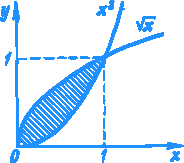
\includegraphics[width=.45\textwidth]{figures/fig-50.pdf} 
\caption{Curvilinear trapezoids as integral of a function.}
\label{fig-50}
\end{figure}

\rdr This area is the difference between the areas
of two curvilinear trapezoids: 
\begin{equation*}%
S = \int_{0}^{1} \sqrt{x} \, dx -  \int_{0}^{1} x^{2} \, dx
\end{equation*}
Therefore,
\begin{equation*}%
S = \dfrac{2}{3} x \sqrt{x} |_{0}^{1} -  \dfrac{1}{3} x^{3} |_{0}^{1} = \dfrac{2}{3} 	 - \dfrac{1}{3} = \dfrac{1}{3}
\end{equation*}

\athr Correct. Consider another example. Find the area of the shaded figure in	\fig{fig-51}.

\begin{figure}[!ht]%[13]{r}{0.5\textwidth}
\centering
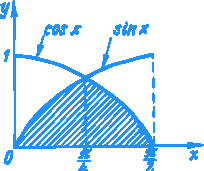
\includegraphics[width=.45\textwidth]{figures/fig-51.pdf}
\caption{Curvilinear trapezoid as the integral of a function.}
\label{fig-51}
\end{figure}

\rdr The graphs of the functions $\sin x$ and $\cos x$ intersect at the point $x = \dfrac{\pi}{4}$. Consequently, one has to use the antiderivative of the function $\sin x$ over the interval $\left[ 0, \, \dfrac{\pi}{4} \right]$ and that of the function $\cos x$ over the interval $\left[  \dfrac{\pi}{4}, \, \dfrac{\pi}{2} \right]$. Hence,
\begin{align*}%
S & = \int_{0}^{\frac{\pi}{4}} \sin x \, dx + \int_{\frac{\pi}{4}}^{\frac{\pi}{2}} \cos x \, dx  = - \cos x |_{0}^{\frac{\pi}{4}}  + \sin x |_{\frac{\pi}{4}}^{\frac{\pi}{2}} \\
& = - \left(\cos \frac{\pi}{4} - \cos 0 \right) + \left(\sin \frac{\pi}{2} - \sin \frac{\pi}{4}  \right) \\
& = - \left( \frac{\sqrt{2}}{2} - 1 \right) + \left(1 - \frac{\sqrt{2}}{2}  \right) \\
& = 2 - \sqrt{2}
\end{align*}

\athr Perfectly right. Now we shall discuss one ``fine point'', returning to formula \eqref{newton-lebnitz-formula} and rewriting it in the form
\begin{equation}%
\boxed{\int_{a}^{x} f(t) \, dt = F(x)- F(a)}
\label{newton-lebnitz-formula2}
% eq 2 of 12
\end{equation}
What has been changed by this rewriting? 

\rdr First, we have replaced the \emph{constant} upper limit of integration (the number $b$) by the \emph{variable} limit of integration (the variable $x$). Second, we have substituted the integration variable $t$ for the integration variable $x$.

\athr Only the first of these changes is significant. The second (the substitution of the integration variable) is of no consequence. It is easy to see that the formulas
\begin{equation*}%
\int_{a}^{b} f(x) \, dx \,\, \int_{a}^{b} f(t) \, dt \,\, \int_{a}^{b} f(y) \, dy \,\, \int_{a}^{b} f(z) \, dz
\end{equation*}
are \emph{equivalent} since all the four give $F (b) - F (a)$. So it does not matter what \emph{symbol} is used for the integration variable in each particular case.

\rdr Why, then, did you have to substitute the variable $t$ for the integration variable $x$ in \eqref{newton-lebnitz-formula2}?

\athr Only not to confuse the integration variable with the variable upper limit. These are different variables and, of course, must be denoted by different symbols.
The expression
\begin{equation*}%
\int_{a}^{x} f(t) \,\, dt
\end{equation*}
is called the \emph{integral with a variable upper limit}. It is important that in contrast to the expression
\begin{equation*}%
\int_{a}^{b} f(t) \,\, dt
\end{equation*}
this expression yields not a number but a function. According to \eqref{newton-lebnitz-formula2}, this function is $F (x) - F (a)$.

\rdr But if the $\displaystyle\int_{a}^{b} \Box dt$ ``black box'' is a \emph{functional}, then the $\displaystyle\int_{a}^{x} \Box dt$ ``black box'' is an operator? (I have used
here our symbolic notation of ``windows'' into which the function $f$ must be input).

\athr Correct. This is immediately clear in the following unusual table.

\begin{center}
\textcolor{DodgerBlue}{\textbf{An Unusual Table}}\\[20pt]
%{\smaller
\boxed{
\begin{tabular}{>{\color{IndianRed}}c>{\color{IndianRed}}c>{\color{IndianRed}}c}
%\toprule
   $f(x)$ & $\int_{1}^{2} f(t) \,\, dt$ &  $\int_{1}^{x} f(t) \,\, dt$ \\
    \arrayrulecolor{DodgerBlue} \toprule
$2x$ & 3 & $x^{2} -1 $\\
\midrule
$3x^{2}$ & 7 & $x^{3} -1 $\\
\midrule
$4x^{3}$ & 15 & $x^{4} -1 $\\
\midrule
$5x^{4}$ & 31 & $x^{5} -1 $\\
\midrule
$6x^{5}$ & 63 & $x^{6} -1 $
\end{tabular}
}
\end{center}
The second and third columns of this table show \emph{what} the
``output'' of the two ``black boxes'',  $\displaystyle\int_{1}^{2} f(t) \,\, dt$ and  $\displaystyle\int_{1}^{x} f(t) \,\, dt$, is when the ``input'' is a function $f$ of the first column.

The integral $\displaystyle\int_{a}^{x} (\ldots) \,\, dt$ is thus indeed an operator. Note that its effect on a function is \emph{opposite} to that of the operator $\ddx$ (we discussed this operator in Dialogue Nine).

Indeed, take a function $f$ and first apply to it the operator $\displaystyle\int_{a}^{x} (\ldots) \,\, dt$ and then the operator $\ddx: \,\, \ddx \left( \displaystyle\int_{a}^{x} (\ldots) \,\, dt \right) $.
This gives
\begin{equation*}%
\ddx \left( \int_{a}^{x} (\ldots) \,\, dt \right) = \ddx [F(x) - F(a)]  = \ddx F(x) = f(x)	
\end{equation*}
i.e. we obtain the initial function $f$. 

\rdr We could apply these operators to the function in the \emph{reverse} order, couldn't we?

\athr Yes, we could. This means that the expression
\begin{equation*}%
 \int_{a}^{x} \left( \dfrac{d}{dt} f(t) \right) \,\, dt
\end{equation*}
also gives the initial function $f$. At least, to within a constant term.

\rdr Can it be verified?

\athr Yes, and very easily. What function is the antiderivative for $f' (x)$?

\rdr Obviously, the function $f (x) + c$. 

\athr Therefore,
\begin{equation*}%
 \int_{a}^{x} \left( \dfrac{d}{dt} f(t) \right) \,\, dt =  \int_{a}^{x} f'(t) \,\, dt = f(x) - f(a)
\end{equation*}

\rdr Will it be correct to say that while the operator $\ddx$ performs the \emph{operation of differentiation}, the operator $\displaystyle\int_{a}^{x} (\ldots) \,\, dt$ performs the \emph{operation of integration}?

\athr Precisely. It might seem that the topic is exhausted, but the discussion would be incomplete without a clarification of one essential ``subtlety''. Throughout this dialogue we operated with something we called ``the area of a curvilinear trapezoid'' and found that this is the meaning of the integral. But what is the ``area of a curvilinear trapezoid?''

\rdr But surely this is self-evident. One glance at the figures is enough.

\athr Look, for instance, at \fig{fig-45}. It shows a shaded geometrical figure called a curvilinear trapezoid. But it says nothing about the \emph{area} of the trapezoid.

\rdr The area is a standard concept in geometry.

\athr No objections. But do not forget that in geometry you normally apply this concept to a well-defined set of figures: triangles, trapezoids, etc. And you remember that difficulties arise when you try to determine the \emph{area of a circle}. By definition, the area of a circle is the limit of the sequence of the areas of regular polygons inscribed in, or circumscribed around, the circle, for an infinitely increasing number of the sides of the polygon.

\rdr Presumably, the area of a curvilinear trapezoid can also be defined as the \emph{limit of a specific sequence of areas}? 

\athr Yes, this is the normal approach. Consider a curvilinear trapezoid bounded by the graph of a function $f (x)$ over the interval $[a, b]$ (\fig{fig-52}). Let us subdivide the interval $[a, b]$ into n subintervals of identical length $\Delta x = \dfrac{b-a}{n}$ (in \fig{fig-52} $n = 10$). The end points of these n
subintervals are denoted from left to right: 
\begin{equation*}%
x_{0} = a, \, x_{1}, \, x_{2}, \,x_{3}, \, \ldots x_{n} = b
\end{equation*}
On each $\Delta x$-long interval, used as a base, we construct a \emph{rectangle} of altitude $f (x_{k-1})$, where $k$ is the subscript of the right-hand end of this subinterval (this choice is arbitrary; the left-hand end would do equally well). The area of this rectangle is
\begin{equation*}%
f (x_{k-1}) \, \Delta x
\end{equation*}
Consider now a sum of the areas of all such rectangles (this
total area is shaded in \fig{fig-52}): 
\begin{align*}%
S_{n} (a, b) & = f(x_{0}) \Delta x +  f (x_{1}) \Delta x + \ldots + f (x_{n-1}) \Delta x \\
& = [f(x_{0})  +  f (x_{1})  + \ldots + f (x_{n-1})] \,\, \dfrac{b-a}{ n}
\end{align*}
As the function $f (x)$ is continuous, the ensemble of all these rectangles for sufficiently large $n$ (sufficiently small $\Delta x$) will be very close to the curvilinear trapezoid in question, and, at any rate, the closer the larger $n$ is (the smaller $\Delta x$). It is, therefore, logical to assume the following definition:

\begin{figure}[!ht]%[13]{r}{0.5\textwidth}
\centering
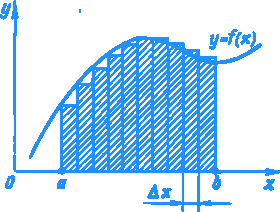
\includegraphics[width=.6\textwidth]{figures/fig-52.pdf} 
\caption{Curvilinear trapezoids as integral of a function.}
\label{fig-52}
\end{figure}

\begin{mytheo}{Definition:}
The sequence of sums $(S_{n} (a, b))$ with $n$ tending to infinity has the limit said to be the area of the given curvilinear trapezoid $S (a, b)$:
\begin{equation}%
S(a,b)= \lmts{n}{\infty} S_{n} (a, \, b)
\label{area-of-trapezoid}
% eq 3 of 12
\end{equation}
\end{mytheo}

\rdr The area $S (a, b)$ of a curvilinear trapezoid was shown earlier to be the integral $\displaystyle\int_{a}^{b} f(x) \,\, dx$; consequently, definition \eqref{area-of-trapezoid} is a new definition of the integral:
\begin{equation}%
\boxed{\int_{a}^{b} f(x) \, dx = \lmts{n}{\infty} S_{n} (a, \, b)}
\label{int-def-2}
% eq 4 of 12
\end{equation}
Do you agree? 

\athr Yes, certainly. And note that definition \eqref{int-def-2}
is \emph{independent}, that is, it is not based on the concept of the antiderivative.

Historically, by the way, the integral appeared as \eqref{int-def-2}, the fact that explains the origin of the standard notation. Indeed, if definition \eqref{int-def-2} is rewritten in a slightly different form
\begin{equation}%
\int_{a}^{b} f(x) \, dx = \lmts{n}{\infty} \left( \sum_{k=1}^{n} f(x_{k-1}) \Delta x \right)
\label{int-def-3}
% eq 5 of 12
\end{equation}
you may notice a certain similarity in the form of the left- and right-hand sides of this equality. The very symbol $\int$( the integral sign) originated from the letter $S$ which was often used to denote sums. The product $f(x_{k-1}) dx$ evolved to $f (x) dx$. In the 17th century mathematicians did not use the concept of the limit. They treated integrals as ``sums of an infinitely large number of infinitely small addends'', with $f (x) dx$ being these infinitesimal addends. In this sense, the area of a curvilinear trapezoid $S$ was defined as the ``sum of an infinitely large number of infinitely small areas $f (x) dx$.''

You realize, I hope, that such concepts were obviously lacking mathematical rigorousness.

\rdr This illustrates what you termed on many occasions ``subjective impressions''.

\athr It must be clear to you by now that a strict mathematical interpretation of the concept of the \emph{integral} is possible only if the \emph{limit transition} is used. I have already emphasized that the limit transition is the foundation of calculus. If the concept of the limit is avoided (``limit of sequence'' or ``limit of function''), neither the derivative nor integral can he treated rigorously.

\rdr But the integral can be defined without resorting to  \eqref{int-def-2}. It is quite sufficient to use the Newton-Leibnitz formula \eqref{newton-lebnitz-formula}. And this formula does not involve any limit transitions.

\athr But this formula involves the antiderivative. And the antiderivative involves, in the long run, the concept of the derivative, that is, the unavoidable limit transition.

By the way, your last remark makes me touch the aspects of introducing the integral in the literature. Two methodically distinct approaches are possible. 

The \emph{first approach} (the one used in those dialogues) assumes
that the operation of integration is directly introduced as an operation inverse to differentiation. The Newton-Leibnitz formula \eqref{newton-lebnitz-formula} then serves, in fact, as the definition of the integral: it is defined as an \emph{increment of the anti-derivative}.

The \emph{second approach} assumes that the operation of integration is introduced as an \emph{independent} operation, the integral being defined as the \emph{limit} of a sequence formed of the appropriate sums (see formula  \eqref{int-def-2}). This approach corresponds to the historical progress in mathematics; indeed, originally integral calculus was evolving independently of differential calculus. The profound relationship between the two branches of mathematics had been discovered only by the end of the 17th century when the main problems of the two were understood as \emph{mutually inverse}. The Newton-Leibnitz formula \eqref{newton-lebnitz-formula} was precisely a reflection of this relationship: it was demonstrated that the integral is none other than an increment of the antiderivative.